\documentclass{article}

\usepackage{graphicx}
\usepackage{tikz}
\usepackage{tikzsymbols}
\usetikzlibrary{calc,patterns,shapes.geometric}
\pagestyle{empty}
\usepackage[margin=0pt]{geometry}
\geometry{papersize={14in,12in}}

\def\centerarc[#1](#2)(#3:#4:#5){\draw[#1] ($(#2)+({#5*cos(#3)},{#5*sin(#3)})$) arc (#3:#4:#5);}

\begin{document}
	\begin{figure}
		\centering
		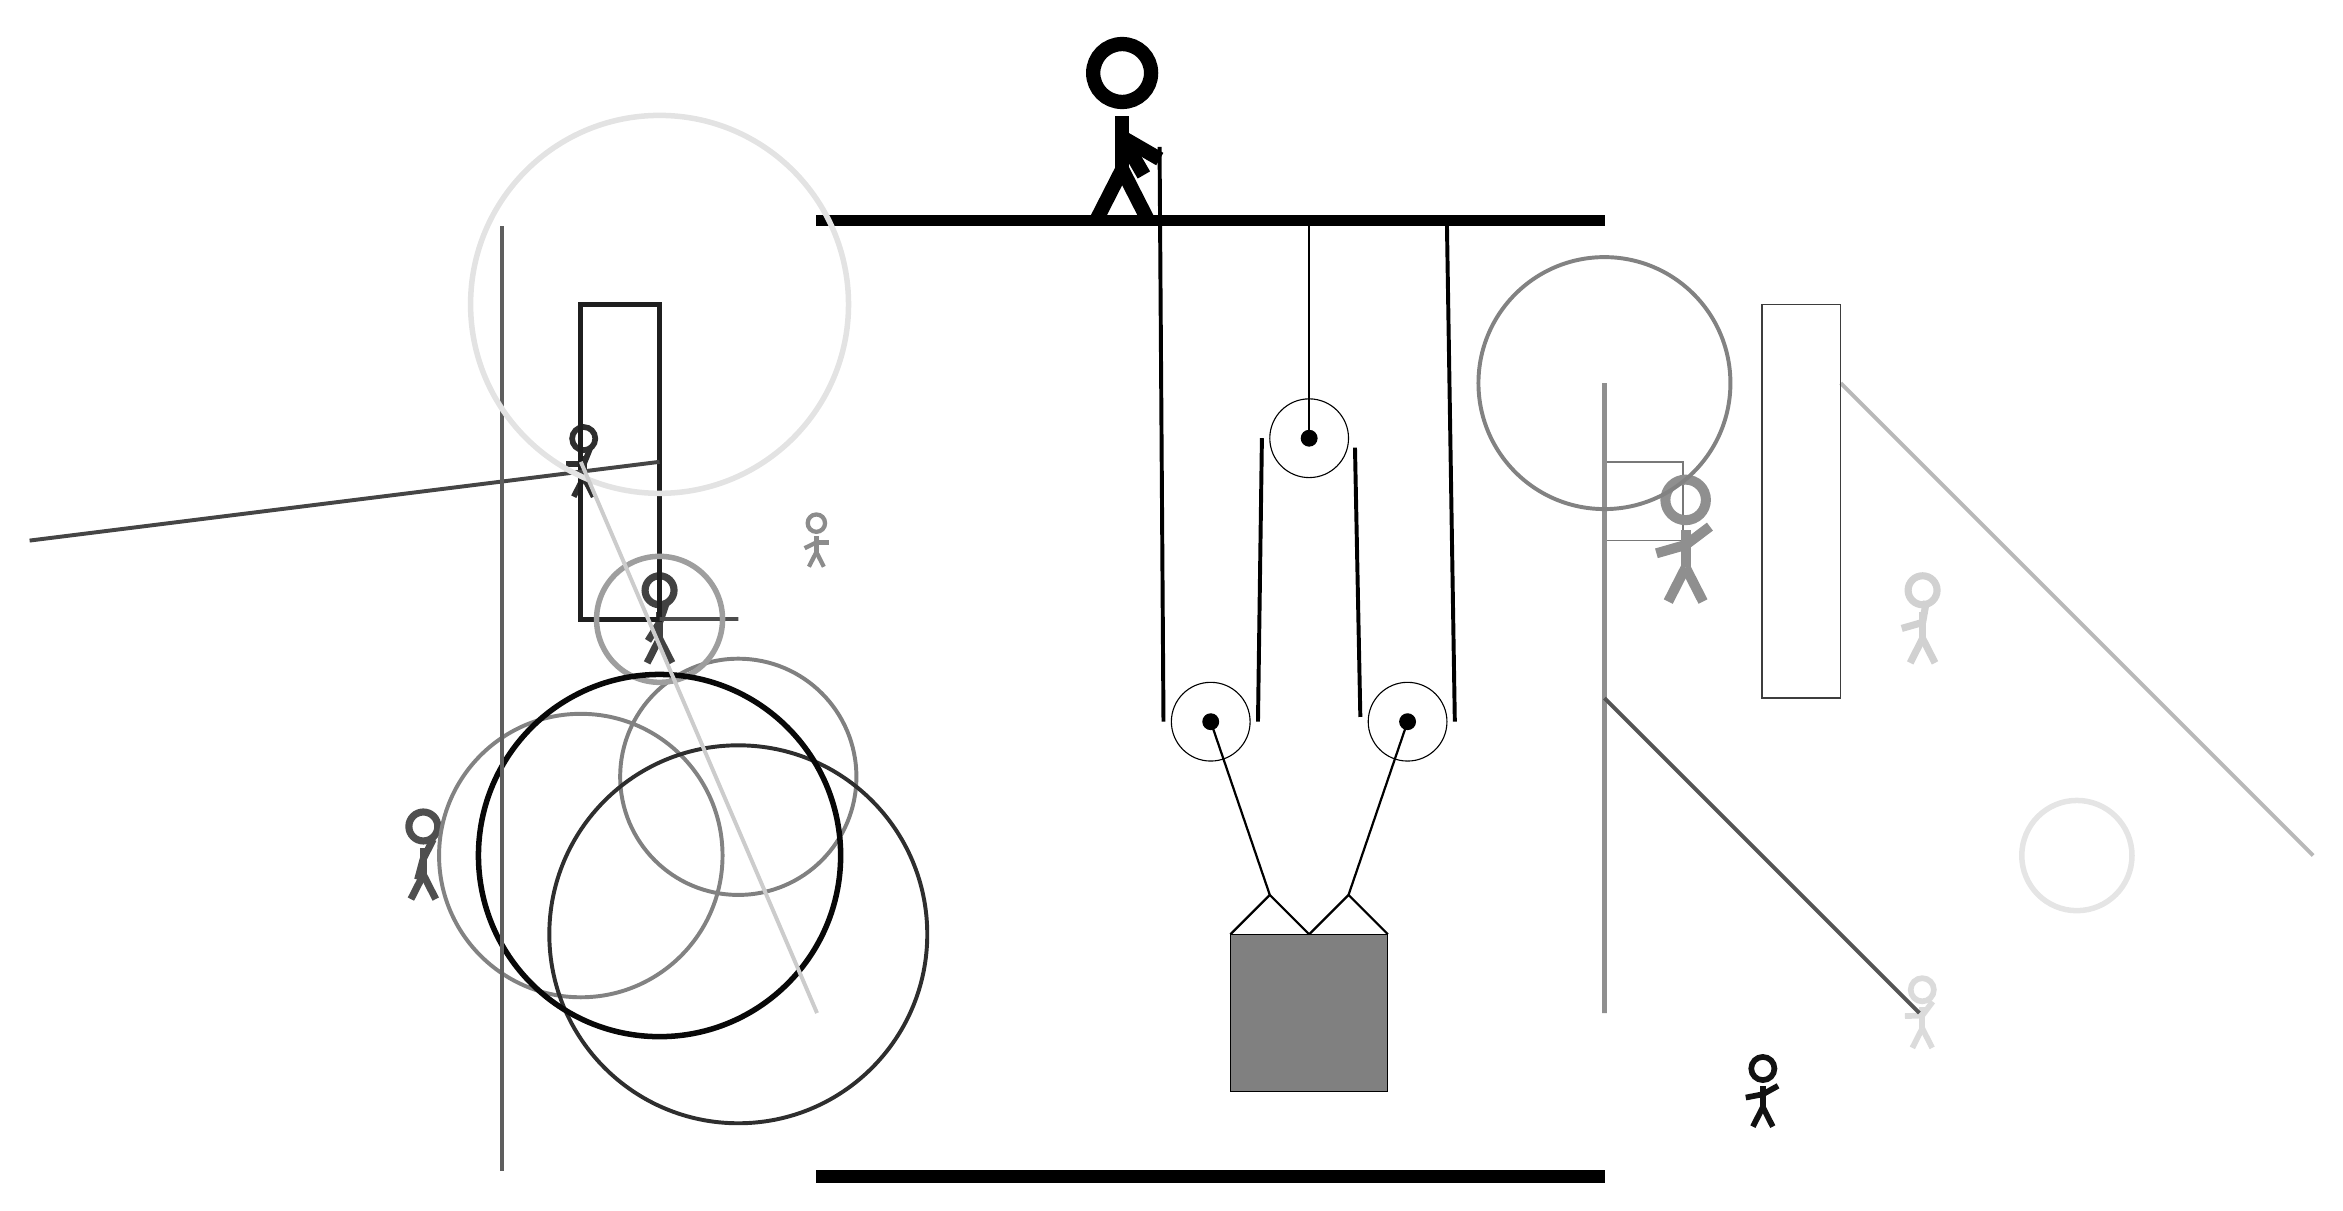
\begin{tikzpicture}
			%%%%% START %%%%%
			
			\draw[fill=black] (-4, 9) rectangle (6, 9.125);
			
			\draw (1, 2.7) circle (0.5);
			\draw[fill=black] (1, 2.7) circle (0.1);
			
			\draw (2.25, 6.3) circle (0.5);
			\draw[fill=black] (2.25, 6.3) circle (0.1);
			\draw[thick] (2.25, 6.3) -- (2.25, 9);
			
			\node[line width=0.2mm, color=black!82] at (-7, 6) {\Strichmaxerl[4][0][68]};
			
			\node[line width=0.3mm, color=black!93] at (8, -2) {\Strichmaxerl[4][11][29]};
			\draw [line width=0.5mm, color=black!80](12, 1) circle (0.0);
			\node[line width=0.2mm, color=black!69] at (-9, 1) {\Strichmaxerl[5][75][63]};
			\node[line width=0.6mm, color=black!74] at (-6, 4) {\Strichmaxerl[5][58][71]};
			
			\draw [line width=0.5mm, color=black!50](-5, 2) circle (1.5);
			\draw [line width=0.5mm, color=black!49](-7, 1) circle (1.8);
			\node[line width=0.3mm, color=black!45] at (-4, 5) {\Strichmaxerl[3][26][0]};
			\draw[line width=0.2mm, color=black!53] (6, 5) rectangle (7, 6);
			\node[line width=0.2mm, color=black!14] at (10, -1) {\Strichmaxerl[4][2][53]};
			\draw[line width=0.7mm, color=black!44] (6, -1) rectangle (6, 7);
			\draw[line width=0.5mm, color=black!28](9, 7) -- (15, 1);
			\node[line width=0.7mm, color=black!44] at (7, 5) {\Strichmaxerl[7][16][37]};
			\draw [line width=0.5mm, color=black!49](6, 7) circle (1.6);
			\draw [line width=0.5mm, color=black!82](-5, 0) circle (2.4);
			\draw[line width=0.5mm, color=black!67](10, -1) -- (6, 3);
			\draw[line width=0.6mm, color=black!88] (-6, 8) rectangle (-7, 4);
			\draw[line width=0.5mm, color=black!70] (-5, 4) rectangle (-6, 4);
			\draw [line width=0.7mm, color=black!10](12, 1) circle (0.7);
			\node[line width=0.7mm, color=black!18] at (10, 4) {\Strichmaxerl[5][16][80]};
			\draw [line width=0.7mm, color=black!38](-6, 4) circle (0.8);
			\draw[line width=0.5mm, color=black!73](-6, 6) -- (-14, 5);
			
			\draw [line width=0.7mm, color=black!97](-6, 1) circle (2.3);
			\draw[line width=0.5mm, color=black!63](-8, -3) -- (-8, 9);
			\draw [line width=0.7mm, color=black!11](-6, 8) circle (2.4);
			
			\draw[line width=0.2mm, color=black!76] (8, 8) rectangle (9, 3);
			\draw[line width=0.5mm, color=black!20](-7, 6) -- (-4, -1);
			
			\draw (3.5, 2.7) circle (0.5);
			\draw[fill=black] (3.5, 2.7) circle (0.1);
			
			\draw[thick] (3.5, 2.7) -- (2.75, 0.5);
			\draw[thick] (1, 2.7) -- (1.75, 0.5);
			\draw[thick]  (1.25, 0) -- (1.75, 0.5) -- (2.25, 0);
			\draw[thick]  (2.25, 0) -- (2.75, 0.5) -- (3.25, 0);
			\draw[fill=black!50] (1.25, 0) rectangle (3.25, -2);
			
			\draw[line width=0.5mm] (0.35, 10) --  (0.4, 2.7);
			\centerarc[line width=0.5mm](1, 2.7)(180:360:0.6);
			\draw[line width=0.5mm] (1.6, 2.7) -- (1.65, 6.3);
			\centerarc[line width=0.5mm](2.25, 6.3)(-20:180:0.6);
			\draw[line width=0.5mm](2.832, 6.18) -- (2.9, 2.76);
			\centerarc[line width=0.5mm](3.5, 2.7)(160:360:0.6);
			\draw[line width=0.5mm](4.1, 2.7) -- (4.0, 9);
			
			\node at (-0.07, 10.2) {\Strichmaxerl[10][120][-30]};
			
			\draw[fill=black] (-4, -3) rectangle (6, -3.15);
			
			%%%%% END %%%%%
		\end{tikzpicture}
	\end{figure}	
\end{document}